Maps are scale models of the earth by itself. Scaling is a simple concept per se, but is complicated by the earth's curvature. It will control multiple things e.g. how many data can be mapped in a map frame, the size of symbols, the overlap of symbols, and so forth \iacite{Longley2005}. Without considering curvature, scaling can be explained as the reduction or enlargement of real world objects by a constant amount.

The following list shows two different representations of scales:
\begin{enumerate}
\ditem{Bar scale} \hfill \\
Figure \ref{fig:bar-scale} on page \pageref{fig:bar-scale} visually shows the scale of a map. The first black bar indicates, that $1$cm in the map represents $100$cm in real world. It includes everything needed: the ratio, the unit of measure and a visual example of both.

\begin{figure}[!htb]
\centering
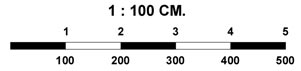
\includegraphics[width=0.4\textwidth,keepaspectratio]{images/methods/scalebar.jpg}
\caption[
    Bar scale.
]{Bar scale.}
\label{fig:bar-scale}
\end{figure}

\ditem{Lexical scale} \hfill \\
Words describing a ratio are known as lexical scales. $1:1000$ can be interpreted as as scale, where $1$ unit of measure on the map, represents $1000$ units of measure in real world. The unit of measure is very important to mention in a lexical scale.
\end{enumerate}

However, taking the earth's curvature into consideration, scaling large areas result in noticeable distortions. The distribution of distortion is dependent on the map projection (see chapter \ref{s:map-projections} on page \pageref{s:map-projections} for more information).

Choosing the correct type of scale depends on several factors: the theme and purpose of the map, data resolution and the specified format. If a map is designed for navigation, it will need more detail than if it is designed to show an overview of a national park \iacite{Tyner2010}.